\chapter{Análisis y Trazado de las Rectas de Carga}
\label{chap:rectas_de_carga}

El análisis gráfico mediante rectas de carga permite visualizar de forma directa la interacción entre el circuito de
polarización en continua y la respuesta dinámica en alterna frente a señales de gran y pequeña amplitud, verificando
los márgenes reales de excursión simétrica sin distorsión por recorte.

\section{Recta de Carga Estática de Corriente Continua}

La recta de carga estática (CC) modela el comportamiento de la malla de salida en reposo, donde los capacitores de
bloqueo y desacoplo se comportan como circuitos abiertos. La ecuación de malla viene dada por:
\begin{equation}
  V_{CC} = v_{CE} + i_C \cdot R_{CC}
\end{equation}
donde $R_{CC} = R_C + R_E = 1380\ohm$. Despejando la corriente de colector en función de la tensión colector-emisor:
\begin{equation}
  i_C = -\frac{1}{R_{CC}} \cdot v_{CE} + \frac{V_{CC}}{R_{CC}}
  \label{eq:recta_cc}
\end{equation}

Los puntos de intersección con los ejes coordenados son:
\begin{enumerate}
  \item Intersección con el eje de abscisas (tensión de corte en continua, $i_C = 0$):
    \begin{equation}
      V_{CE,\text{corte(CC)}} = V_{CC} = 15.00\V \implies (15\V,\, 0\mA)
    \end{equation}
  \item Intersección con el eje de ordenadas (corriente de saturación en continua, $v_{CE} = 0$):
    \begin{equation}
      I_{C,\text{sat(CC)}} = \frac{V_{CC}}{R_{CC}} = \frac{15\V}{1380\ohm} \approx 10.87\mA \implies (0\V,\, 10.87\mA)
    \end{equation}
\end{enumerate}

Esta recta posee una pendiente negativa de $m_{CC} = -1/R_{CC} \approx -7.246 \times 10^{-4}\,\Omega^{-1}$.

\section{Recta de Carga Dinámica de Corriente Alterna}

A la frecuencia de trabajo de la señal ($1\kHz$), los capacitores $C_1, C_2$ y $C_E$ presentan reactancias despreciables,
actuando efectivamente como cortocircuitos. De este modo, la carga vista por el colector en alterna es $R_{CA} = R_C \parallel R_L = 545.45\ohm$.

La ley de variación dinámica alrededor del punto de reposo $Q(V_{CEQ}, I_{CQ})$ impone:
\begin{equation}
  i_C - I_{CQ} = -\frac{1}{R_{CA}} \cdot (v_{CE} - V_{CEQ})
\end{equation}
reescribiéndose en forma explícita:
\begin{equation}
  i_C = -\frac{1}{R_{CA}} \cdot v_{CE} + \left(I_{CQ} + \frac{V_{CEQ}}{R_{CA}}\right)
  \label{eq:recta_ca}
\end{equation}

A partir del punto de trabajo normalizado verificado en el software de cálculo y GeoGebra, $Q(V_{CEQ} = 4.46\V,\, I_{CQ} = 7.64\mA)$,
se obtienen los puntos notables de la recta dinámica:
\begin{enumerate}
  \item Tensión de corte dinámica ($i_C = 0$):
    \begin{equation}
      V_{CE,\max(\text{CA})} = V_{CEQ} + I_{CQ} \cdot R_{CA} = 4.46\V + (7.64\mA \cdot 545.45\ohm) = 4.46\V + 4.167\V \approx 8.627\V
    \end{equation}
    correspondiente al punto coordenado $(8.627\V,\, 0\mA)$.
  \item Corriente de saturación dinámica ($v_{CE} = 0$):
    \begin{equation}
      I_{C,\max(\text{CA})} = I_{CQ} + \frac{V_{CEQ}}{R_{CA}} = 7.64\mA + \frac{4.46\V}{545.45\ohm} = 7.64\mA + 8.177\mA \approx 15.82\mA
    \end{equation}
    correspondiente al punto coordenado $(0\V,\, 15.82\mA)$.
\end{enumerate}

La pendiente de la recta dinámica resulta notablemente más pronunciada: $m_{CA} = -1/R_{CA} \approx -1.833 \times 10^{-3}\,\Omega^{-1}$.

\section{Gráfico de las Rectas de Carga y Excursión Simétrica}

En la figura~\ref{fig:rectas_carga} se exhibe el gráfico generado en GeoGebra donde se representan de forma conjunta
la recta estática de continua (trazo verde), la recta dinámica de alterna (trazo rojo) y la ubicación del punto de
operación $Q$.

\begin{figure}[!ht]
  \centering
  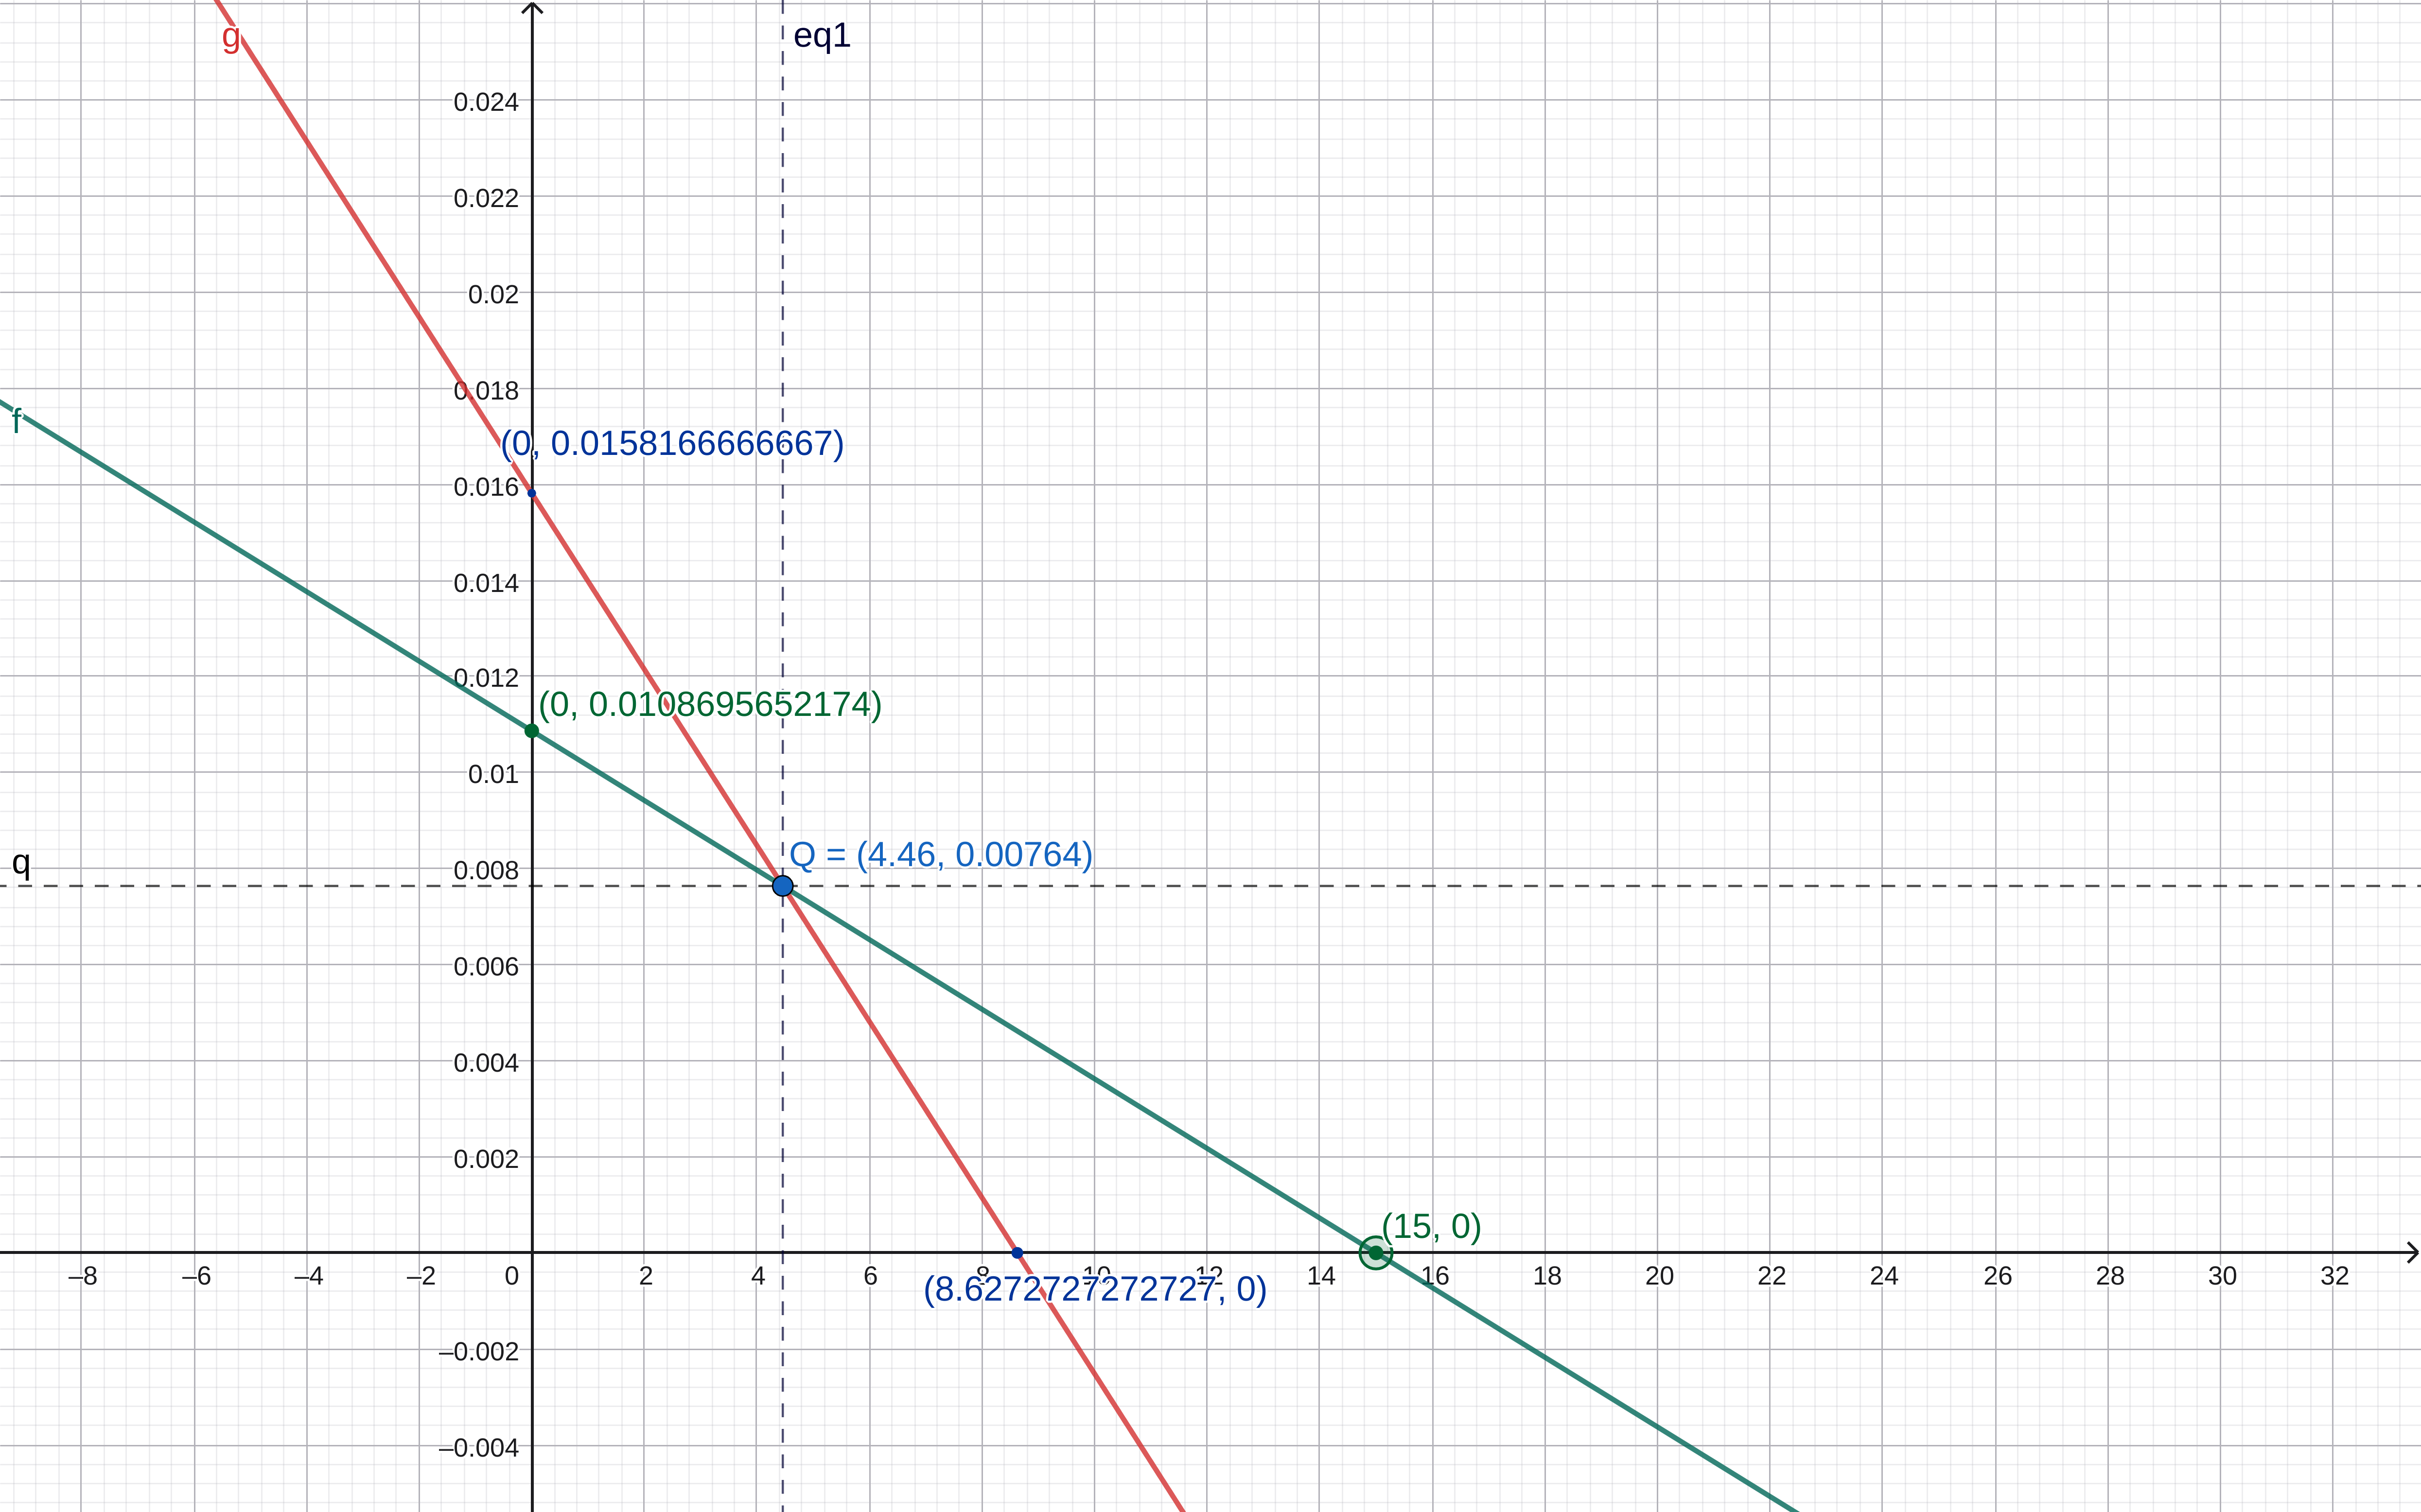
\includegraphics[width=0.92\textwidth]{images/rectas_carga.png}
  \caption{Gráfico de las rectas de carga estática y dinámica en el plano $i_C - v_{CE}$ obtenido en GeoGebra.}
  \label{fig:rectas_carga}
\end{figure}

A partir de la posición relativa del punto $Q$ sobre la recta de carga dinámica, se analizan los márgenes de excursión:
\begin{itemize}
  \item Margen de tensión hacia el corte:
    \begin{equation}
      \Delta v_{CE,\text{corte}} = V_{CE,\max(\text{CA})} - V_{CEQ} = 8.627\V - 4.46\V = 4.167\V
    \end{equation}
  \item Margen de tensión hacia la saturación (considerando $V_{CE,\text{sat}} \approx 0.2\V$):
    \begin{equation}
      \Delta v_{CE,\text{sat}} = V_{CEQ} - V_{CE,\text{sat}} = 4.46\V - 0.20\V = 4.26\V
    \end{equation}
\end{itemize}

El límite inferior determina la máxima amplitud pico admisible para la señal de salida sin incurrir en recorte ni
distorsión no lineal:
\begin{equation}
  \hat{v}_{o,\max} = \min(\Delta v_{CE,\text{corte}},\, \Delta v_{CE,\text{sat}}) = 4.167\V
\end{equation}
lo que define una capacidad de excursión simétrica pico a pico máxima sobre la carga de:
\begin{equation}
  v_{o,pp,\max} = 2 \cdot \hat{v}_{o,\max} \approx 8.33\V_{pp}
\end{equation}

En las pruebas experimentales de laboratorio se excitó el amplificador con una amplitud suficiente para obtener una
tensión de salida de $v_L = 1.30\V_{pp}$ (como se aprecia en la pantalla del osciloscopio). Al verificarse que
$1.30\V_{pp} \ll 8.33\V_{pp}$, el circuito operó holgadamente dentro de su rango dinámico lineal, garantizando una forma
de onda senoidal pura y libre de distorsiones armónicas apreciables.
